\documentclass[sigconf,9pt]{acmart}
\usepackage{graphicx}
\usepackage{booktabs}
\usepackage{subcaption}
\usepackage{placeins}
\usepackage{dblfloatfix}
\usepackage{afterpage}
\usepackage{tabularx}
\usepackage{array}
\usepackage{tikz}
\usetikzlibrary{positioning,arrows.meta,fit,backgrounds,calc}
\newcolumntype{C}{>{\centering\arraybackslash}X}
\newcolumntype{R}{>{\raggedleft\arraybackslash}X}

% diagram styles
\tikzset{
  blk/.style={draw=black!65, rounded corners=2pt, fill=#1, align=center,
              font=\fontsize{7.2}{8.4}\selectfont, inner sep=3pt},
  arr/.style={-{Stealth[length=1.8mm]}, thick, black!70}
}

%% Rights & Conference Info (MobiSys '26)
\copyrightyear{2026}
\acmYear{2026}
\setcopyright{cc}
\setcctype{by}
\acmConference[MobiSys Companion '26]{The 24th Annual International Conference on Mobile Systems, Applications and Services}{June 21--25, 2026}{Cambridge, United Kingdom}
\acmBooktitle{The 24th Annual International Conference on Mobile Systems, Applications and Services (MobiSys Companion '26), June 21--25, 2026, Cambridge, United Kingdom}
\acmDOI{10.1145/3812835.3814864}
\acmISBN{979-8-4007-2711-5/2026/08}

\begin{document}

\title{Poster: SurakshaNet: Privacy-First, Edge-Deployed Multilingual Abusive Language Detection}

\author{Aamod Jain$^{*}$}
\affiliation{%
  \institution{Indian Institute of Technology Ropar}
  \city{Punjab}
  \country{India}
}
\email{2023csb1092@iitrpr.ac.in}
\author{Pratham Garg$^{*}$}
\affiliation{%
  \institution{Indian Institute of Technology Ropar}
  \city{Punjab}
  \country{India}
}
\email{2023csb1147@iitrpr.ac.in}
\author{Geeta Yadav}
\affiliation{%
  \institution{Indian Institute of Technology Ropar}
  \city{Punjab}
  \country{India}
}
\email{geeta@iitrpr.ac.in}

\begin{abstract}
Cloud moderation APIs raise privacy concerns and add network latency. \textit{SurakshaNet} is a Chrome extension that classifies incoming WhatsApp Web messages on the device with an INT8-quantized multilingual MiniLM running in ONNX Runtime Web; no message text is sent to a server. Dynamic INT8 quantization reduces the model from 470.6\,MB to 118.4\,MB (about 75\%) and changes test accuracy by at most 0.15 points (86.5\% on a mixed Hindi, English and Hinglish test set). A rolling-window gate raises detection of abuse split across several messages on a Hinglish test set from 28.9\% to 76.1\%. We then build a 105{,}000-thread synthetic dataset (English, Hindi, Hinglish; 3--10 messages; five classes) with Qwen3-32B and train five-class thread classifiers. On the synthetic test set a thread-aware MiniLM reaches 97.9\% accuracy (INT8) against 83.2\% when only the last message is used. On real data (CAD, ConvAbuse, PRISM) the same models score only 0.47--0.74 AUROC without fine-tuning, so the synthetic scores do not show real-world accuracy. We describe the data pipeline, training, metrics and limitations.
\end{abstract}

\begin{CCSXML}
<ccs2012>
   <concept>
       <concept_id>10002978.10003022</concept_id>
       <concept_desc>Security and privacy~Software and application security</concept_desc>
       <concept_significance>500</concept_significance>
       </concept>
 </ccs2012>
\end{CCSXML}

\ccsdesc[500]{Security and privacy~Software and application security}
\keywords{Abusive language detection, Privacy-preserving AI, Edge computing, Synthetic data, Conversation threads}
\maketitle
\vspace{-0.5em}
$^{*}$Equal contribution.

%==============================================================
\section{Introduction}
Abusive messages are common on social platforms \cite{Mathew_Saha_Yimam_Biemann_Goyal_Mukherjee_2021}, and women and children are frequent targets. In code-mixed Indian settings (Hindi, Hinglish) \cite{NEURIPS2022_a7c4163b}, abuse can be hard to detect, and sending private chats to a cloud service is often unacceptable. This paper reports what we built and measured, in three parts.

\begin{enumerate}
    \item \textbf{On-device detector (Sections~\ref{sec:system}--\ref{sec:binary}).} A Chrome extension that scores incoming WhatsApp Web messages locally with an INT8 MiniLM (binary: abusive vs.\ non-abusive).
    \item \textbf{Conversation context (Section~\ref{sec:context}).} A rolling window that re-scores short messages together with earlier ones, evaluated on a Hinglish test set and compared with two cloud LLMs on small subsets.
    \item \textbf{Five-class thread dataset and benchmark (Sections~\ref{sec:data}--\ref{sec:external}).} A synthetic dataset of 105{,}000 threads whose label depends on the \emph{earlier} messages, models trained on it, and an honest check on real data.
\end{enumerate}

\par\textbf{What this paper does not claim.} The five-class models are not deployed in the extension, which still uses the binary model. All five-class data are LLM-generated and were checked only by automatic rules, not by human annotators. The synthetic test scores are measured on text from the same generator as the training data. Parental controls, screenshot capture and tamper-evident evidence storage are not part of the build evaluated here (the incident record has a \texttt{screenshot} field that is always empty).

%==============================================================
\section{System Implementation}\label{sec:system}
Figure~\ref{fig:system} shows what runs in the browser. A content script watches the WhatsApp Web page (\texttt{MutationObserver}) and passes each new incoming message and its chat name to a Manifest~V3 service worker. The worker keeps a rolling window of at most 8 turns and 96 content tokens per chat. It scores the message with the INT8 MiniLM through ONNX Runtime Web (WebAssembly). If the chat has earlier turns and the new message has fewer than 8 content tokens, it also scores the joined window and keeps the larger score (the \emph{gate}, Section~\ref{sec:context}). A message is flagged when the score exceeds 0.5, and marked \textit{high} when it is at least 0.9. Flagged messages get a warning banner and are saved to a local incident log in \texttt{chrome.storage.local} (latest 200 incidents). The incident identifier is the SHA-256 of the chat name and message text; we use it only to avoid duplicate entries, not as proof against tampering. Incidents can be exported as JSON or PDF. Model loading is restricted to local files (\texttt{allowRemoteModels} is false), and the code path for inference makes no network request.

\begin{figure*}[!t]
  \centering
  \resizebox{\textwidth}{!}{% Figure 1: what runs inside the browser extension (verified against sw.js, narrative_cache.js, store.js)
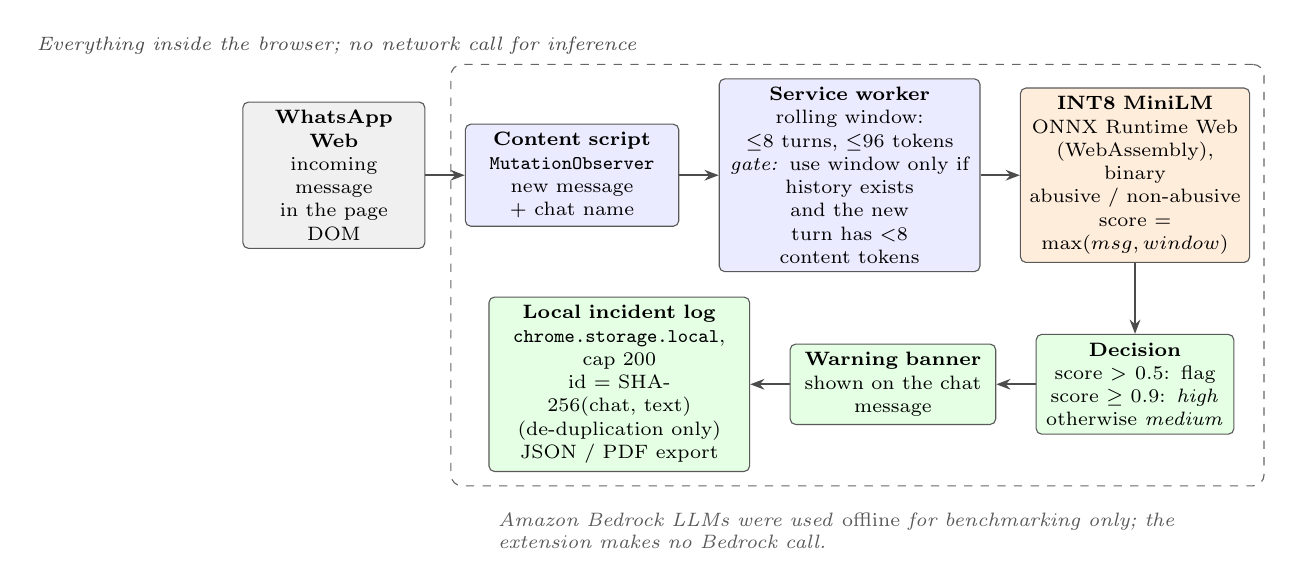
\begin{tikzpicture}[node distance=7mm and 5mm]
  \node[blk=gray!12, text width=2.1cm] (wa) {\textbf{WhatsApp Web}\\incoming message\\in the page DOM};
  \node[blk=blue!8, text width=2.5cm, right=of wa] (cs) {\textbf{Content script}\\\texttt{MutationObserver}\\new message + chat name};
  \node[blk=blue!8, text width=3.1cm, right=of cs] (sw) {\textbf{Service worker}\\rolling window:\\$\le$8 turns, $\le$96 tokens\\\textit{gate:} use window only if\\history exists and the new\\turn has $<$8 content tokens};
  \node[blk=orange!14, text width=2.7cm, right=of sw] (m) {\textbf{INT8 MiniLM}\\ONNX Runtime Web\\(WebAssembly), binary\\abusive / non-abusive\\score $=\max(\text{msg},\text{window})$};
  \node[blk=green!10, text width=2.3cm, below=9mm of m] (dec) {\textbf{Decision}\\score $>0.5$: flag\\score $\ge0.9$: \textit{high}\\otherwise \textit{medium}};
  \node[blk=green!10, text width=2.4cm, left=of dec] (ban) {\textbf{Warning banner}\\shown on the chat\\message};
  \node[blk=green!10, text width=3.1cm, left=of ban] (log) {\textbf{Local incident log}\\\texttt{chrome.storage.local}, cap 200\\id $=$ SHA-256(chat, text)\\(de-duplication only)\\JSON / PDF export};
  \draw[arr] (wa) -- (cs); \draw[arr] (cs) -- (sw); \draw[arr] (sw) -- (m);
  \draw[arr] (m) -- (dec); \draw[arr] (dec) -- (ban); \draw[arr] (ban) -- (log);
  \begin{scope}[on background layer]
    \node[draw=black!60, dashed, rounded corners=4pt, inner sep=5pt, fit=(cs)(sw)(m)(dec)(ban)(log),
          label={[font=\scriptsize\itshape, text=black!70]above left:Everything inside the browser; no network call for inference}] {};
  \end{scope}
  \node[font=\scriptsize\itshape, text=black!65, text width=9cm, align=left, below=4mm of log.south west, anchor=north west]
    {Amazon Bedrock LLMs were used \emph{offline} for benchmarking only; the extension makes no Bedrock call.};
\end{tikzpicture}
}
  \caption{On-device pipeline of the extension. All blocks inside the dashed box run in the user's browser. The cloud LLMs of Section~\ref{sec:context} were used offline for benchmarking only.}
  \label{fig:system}
\end{figure*}

%==============================================================
\section{Binary Detector: Data, Quantization, Accuracy}\label{sec:binary}

\subsection{Training data and protocol}
The shipped model is \texttt{paraphrase-multilingual-MiniLM-L12-v2} \cite{reimers2020multilingual,wang2020minilm} fine-tuned for 3 epochs (1{,}102\,s on a Modal GPU) on three sources (Table~\ref{tab:binary_data}): the Hindi part of MACD \cite{NEURIPS2022_a7c4163b} (human-labelled, ShareChat comments), the Davidson English tweets \cite{davidson2017automated}, and a Hinglish set that we produced by converting MACD Hindi comments into Roman-script, code-mixed Hinglish with a Qwen-based converter. The Hindi split is 60/20/20; Davidson is split 80/10/10. Label 0 is \emph{abusive}.

\begin{table}[h!]
\centering
\caption{Binary training protocol (train / validation / test messages).}
\label{tab:binary_data}
\small
\begin{tabularx}{\linewidth}{@{}l R R R@{}}
\toprule
\textbf{Source} & \textbf{Train} & \textbf{Val} & \textbf{Test} \\
\midrule
Hindi (MACD, human)            & 20{,}183 & 6{,}728  & 6{,}728 \\
English (Davidson, human)      & 19{,}826 & 2{,}478  & 2{,}479 \\
Hinglish (Qwen-converted MACD) & 18{,}920 & 6{,}375  & 6{,}368 \\
\midrule
Total                          & 58{,}929 & 15{,}581 & 15{,}575 \\
\bottomrule
\end{tabularx}
\end{table}

\subsection{INT8 quantization, size and accuracy}
We exported the fine-tuned model to ONNX and applied \emph{dynamic} INT8 quantization (ONNX Runtime/Optimum, AVX2 configuration, per-tensor) \cite{jacob2018quantization}. The weights drop from 448.8\,MiB (470.6\,MB) to a 118.4\,MB file (112.9\,MiB), about 75\% smaller. Table~\ref{tab:quant} compares the FP32 and INT8 models on the held-out test sets: the largest change is $-0.15$ points.

\begin{table}[h!]
\centering
\caption{Test accuracy (\%) of the binary model before and after INT8 quantization.}
\label{tab:quant}
\small
\begin{tabularx}{\linewidth}{@{}l R R R R@{}}
\toprule
\textbf{Test set} & \textbf{$n$} & \textbf{FP32} & \textbf{INT8} & \textbf{$\Delta$} \\
\midrule
Hindi (MACD)    & 6{,}728  & 85.24 & 85.14 & $-0.10$ \\
Hinglish        & 6{,}368  & 84.34 & 84.36 & $+0.02$ \\
English (Davidson) & 2{,}479 & 96.65 & 96.73 & $+0.08$ \\
Mixed (all three) & 15{,}575 & 86.69 & 86.54 & $-0.15$ \\
\bottomrule
\end{tabularx}
\end{table}

\par\textbf{Reference point.} The MACD paper reports 86.34\% accuracy on Hindi for XLM-R pretrained on MACD data \cite{NEURIPS2022_a7c4163b}; our INT8 model scores 85.14\% on Hindi, 1.2 points lower. Both use a 60/20/20 split of MACD Hindi, but we did not re-run their model or check that the splits are identical, and our model also trains on English and Hinglish, so this is only a rough comparison. XLM-R Base has about 270\,M parameters and is much larger than our 118\,MB file.

\par\textbf{Latency.} We measured single-message latency of the shipped INT8 file with native ONNX Runtime on an Apple-silicon laptop CPU (1 thread, batch 1, 300 Hinglish test messages, median 21 tokens): median 5.0\,ms and 95th percentile 16.8\,ms including tokenization. This is a native measurement; we did not re-measure latency inside the browser (WebAssembly), where it will be higher.

%==============================================================
\section{Conversation Context for Hinglish}\label{sec:context}

\subsection{Test set}
Abuse in chats is often spread over several messages. We built four slices from the frozen Hinglish test set: \emph{single message} (6{,}368), \emph{split narrative}, where an abusive sentence is cut over turns (1{,}500; the abusive word is outside the final turn in 1{,}468 of them), \emph{benign chat} (800), and \emph{abuse after small talk} (800). The split-narrative and small-talk slices contain only abusive examples, so accuracy equals recall there.

\par\textbf{Caveat on the Hinglish data.} Our Hinglish text is machine-converted (Hindi $\to$ Hinglish with a Qwen-based converter). Over 31{,}663 converted comments the mean code-mixing index (CMI) is 13.7, and 25.3\% contain no code-mixing at all, whereas the human-written HinGE set (1{,}964 sentences) has a mean CMI of 35.6. Only 21.1\% of our Hinglish test messages pass the $M\ge0.1$, $I\ge0.1$ filter of CodeMixBench \cite{yang-chai-2025-codemixbench}. The Hinglish accuracies in this paper therefore describe converted text and may overstate accuracy on natural Hinglish.

\subsection{Results}
Table~\ref{tab:local_accuracy} compares three ways of using context with the INT8 model: the current message only, the whole chat concatenated, and the gate shipped in the extension (Section~\ref{sec:system}).

\begin{table}[t]
\centering
\caption{Accuracy (\%) of the INT8 model on Hinglish slices.}
\label{tab:local_accuracy}
\small
\begin{tabularx}{\linewidth}{@{}l C C C@{}}
\toprule
\textbf{Slice} & \textbf{Current msg only} & \textbf{Whole chat} & \textbf{Gated (shipped)} \\
\midrule
Single message         & 84.2 & 84.2 & 84.2 \\
Split narrative        & 28.9 & 79.3 & 76.1 \\
Benign chat            & 86.5 & 83.6 & 83.0 \\
Abuse after small talk & 82.4 & 62.3 & 82.9 \\
\bottomrule
\end{tabularx}
\end{table}

Context helps split narratives (28.9\% $\to$ 79.3\% with the whole chat) but concatenating everything hurts abuse after small talk (62.3\%). The gate keeps 76.1\% on split narratives and 82.9\% after small talk, at the cost of more false positives on benign chats (false-positive rate 13.5\% $\to$ 17.0\%). For single messages the abusive-class F1 is 83.6\% with a false-positive rate of 12.9\%.

\subsection{Comparison with cloud LLMs (small subsets)}
We also scored subsets of the same examples with two Amazon Bedrock models (Nova Micro, Qwen3 32B; one-shot prompt, temperature 0, answer ``abusive'' or ``non-abusive''), offline and only for benchmarking. Table~\ref{tab:bedrock_comparison} shows the results (Nova: Nova Micro; Qwen3: Qwen3 32B).

\begin{table}[t]
\centering
\caption{INT8 model vs.\ cloud LLMs on small subsets (percent). $n$ is the subset size; the INT8 model was scored on the same items. ``--'': not scored.}
\label{tab:bedrock_comparison}
\footnotesize
\begin{tabular}{@{}l r r r r@{}}
\toprule
\textbf{Slice} & $n$ & \textbf{INT8} & \textbf{Nova} & \textbf{Qwen3} \\
\midrule
Insult, recall                      & 80 / 50 & 78.0 & 40.8 & 76.0 \\
Mixed set, false-pos.\ rate         & 80      & 20.0 & 3.3  & -- \\
Split, last turn only               & 40 / 20 & 17.5 & 10.0 & 15.0 \\
Split, full window                  & 40 / 20 & 77.5 & 40.0 & 65.0 \\
Benign, false-pos., last turn       & 35      & 5.7  & 8.6  & -- \\
Benign, false-pos., full window     & 35      & 11.4 & 22.9 & -- \\
Small talk, last turn               & 30      & 83.3 & 62.1 & -- \\
Small talk, full window             & 30      & 73.3 & 65.5 & -- \\
\bottomrule
\end{tabular}
\end{table}

Where two sizes are listed, the first is for Nova Micro and the second for Qwen3 32B. With $n$ between 20 and 80, 95\% intervals are roughly $\pm11$ to $\pm22$ points. The gap to Nova Micro on split full-window recall (77.5\% vs.\ 40.0\%, $n{=}40$) is large; the gap to Qwen3 32B ($n{=}20$) is within noise. We conclude only that the small local model is competitive on these slices, not that it beats cloud LLMs in general.

\par\textbf{Learned context cache (not shipped).} We also trained a small key/value cache with a contrastive loss as the context encoder. It raised split-narrative accuracy from 97.9\% to 99.4\%, but accuracy on benign chats fell from 22.3\% to 13.9\%, and single-message accuracy was only 53.8\%--56.4\%. A threshold giving a 15\% false-positive cap restored benign accuracy (88.4\%) but cut split accuracy to 82.9\%. We therefore kept the plain INT8 model with the gate.

%==============================================================
\section{Five-Class Thread Dataset}\label{sec:data}

\subsection{Why a new dataset}
Existing binary data classify one message at a time. The same line (``you are such an idiot'') can be friendly teasing or a real attack depending on the earlier messages, and grooming and harassment are defined by who is talking to whom. We therefore built a dataset in which the \emph{label belongs to the last message given the earlier ones}. There are five classes (Table~\ref{tab:classes}), chosen from prior taxonomies \cite{vanhee2018cyberbullying,guest2021misogyny,banko2020taxonomy,waseem2017understanding,mandl2019hasoc} and aimed at women and children.

\begin{table*}[t]
\centering
\caption{The five classes. The ``last-message rule'' is what the generation prompt asks for.}
\label{tab:classes}
\small
\begin{tabularx}{\textwidth}{@{}l l X X@{}}
\toprule
\textbf{Id and class} & \textbf{Audience} & \textbf{Last-message rule in the prompt} & \textbf{Basis} \\
\midrule
0 benign             & peers, adults, minors & Normal message. Includes hard negatives: parent--child, teacher--student, harmless surprise secrets, consensual flirting. & HASOC non-offensive \cite{mandl2019hasoc} \\
1 friendly\_sarcasm  & peers & Playful, clearly affectionate teasing; the friends are laughing. & Van Hee et al.\ \cite{vanhee2018cyberbullying} \\
2 hostile\_abuse     & peers, adults & Hostile personal insult meant to hurt. Profanity allowed; no slurs about caste, religion, gender, ethnicity or disability; no sexual content. & Waseem et al.\ \cite{waseem2017understanding}, MACD \\
3 sexual\_harassment & adult woman (75\%) or man (25\%) & Unwanted suggestive remark or pressure; not graphic; the target deflects earlier. & Van Hee et al., Guest et al.\ \cite{guest2021misogyny} \\
4 predatory\_grooming & minor (age 10--15, girl or boy) & Secrecy from parents, moving to a private app, meeting alone, parents-away probing, age probing. No sexual content. & Banko et al.\ \cite{banko2020taxonomy} \\
\bottomrule
\end{tabularx}
\end{table*}

\subsection{Generation pipeline}
Figure~\ref{fig:datagen} gives the full flow. We fix a grid of 3 scripts (English, Hindi in Devanagari, Hinglish in Roman letters) $\times$ 4 lengths (3, 5, 7, 10 messages) $\times$ 5 classes, i.e.\ 60 cells with 1{,}750 threads each, 105{,}000 in total. For every thread a seeded sampler picks a class-specific subtype (31 in total, e.g.\ \textit{boss\_employee}, \textit{secrecy\_push}), a topic (40), two names from a pool of 30, the audience, and, where relevant, the target's gender (and the child's age). A prompt built from this scenario asks Qwen3-32B \cite{qwen3} on Amazon Bedrock (temperature 0.85) to return exactly $k$ alternating messages as JSON, each under 30 words, where the last message follows the class rule. Each scenario gets two attempts.

\par\textbf{Validation.} Every generated thread must pass rule-based checks: correct number of turns, no refusal text, turn length, no adjacent duplicates, last line not repeated from the context, correct script (character-ratio and word-list heuristics), no profanity or explicit words outside the hostile class, and no body or photo words in grooming threads. Threads are then de-duplicated by a hash of the normalised text, and a cell is refilled until it has 1{,}750 accepted threads. In the last generation round, 68{,}631 of 69{,}624 attempts (98.6\%) passed; the 993 rejections were profanity in clean classes (352), script mismatch (253), refusals (242), unparsable output (66), sexualised grooming words (76) and 4 others. Generation used about 122{,}000 Bedrock calls and cost an estimated \$22.07. \textbf{No human read or labelled the threads}; the label is the class the prompt asked for, filtered by the rules above.

\begin{figure*}[!t]
  \centering
  \resizebox{\textwidth}{!}{% Figure 2: how the 105,000-thread dataset was generated (verified against dataset_spec.py and build_dataset.py)
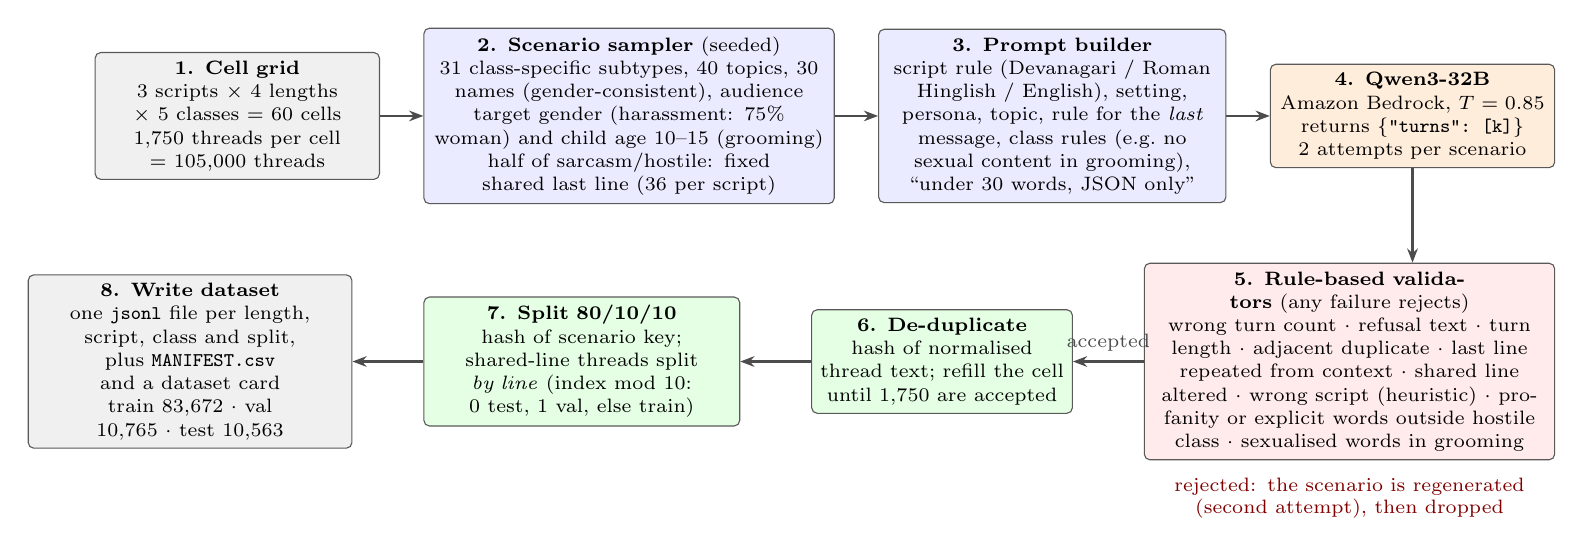
\begin{tikzpicture}[node distance=5.5mm]
  % row 1: build a scenario and ask the LLM
  \node[blk=gray!12, text width=3.4cm] (grid) {\textbf{1. Cell grid}\\3 scripts $\times$ 4 lengths $\times$ 5 classes $=$ 60 cells\\1,750 threads per cell\\$=$ 105,000 threads};
  \node[blk=blue!8, text width=5.0cm, right=of grid] (spec) {\textbf{2. Scenario sampler} (seeded)\\31 class-specific subtypes, 40 topics, 30 names (gender-consistent), audience\\target gender (harassment: 75\% woman) and child age 10--15 (grooming)\\half of sarcasm/hostile: fixed shared last line (36 per script)};
  \node[blk=blue!8, text width=4.2cm, right=of spec] (prompt) {\textbf{3. Prompt builder}\\script rule (Devanagari / Roman Hinglish / English), setting, persona, topic, rule for the \emph{last} message, class rules (e.g.\ no sexual content in grooming), ``under 30 words, JSON only''};
  \node[blk=orange!14, text width=3.4cm, right=of prompt] (llm) {\textbf{4. Qwen3-32B}\\Amazon Bedrock, $T=0.85$\\returns \texttt{\{"turns": [k]\}}\\2 attempts per scenario};
  % row 2 (right to left): check, de-duplicate, split, write
  \node[blk=red!8, text width=5.0cm, below=12mm of llm.south east, anchor=north east] (val) {\textbf{5. Rule-based validators} (any failure rejects)\\wrong turn count $\cdot$ refusal text $\cdot$ turn length $\cdot$ adjacent duplicate $\cdot$ last line repeated from context $\cdot$ shared line altered $\cdot$ wrong script (heuristic) $\cdot$ profanity or explicit words outside hostile class $\cdot$ sexualised words in grooming};
  \node[blk=green!10, text width=3.1cm, left=9mm of val] (dedup) {\textbf{6. De-duplicate}\\hash of normalised thread text; refill the cell until 1,750 are accepted};
  \node[blk=green!10, text width=3.8cm, left=9mm of dedup] (split) {\textbf{7. Split 80/10/10}\\hash of scenario key; shared-line threads split \emph{by line} (index mod 10: 0 test, 1 val, else train)};
  \node[blk=gray!12, text width=3.9cm, left=9mm of split] (out) {\textbf{8. Write dataset}\\one \texttt{jsonl} file per length, script, class and split, plus \texttt{MANIFEST.csv} and a dataset card\\train 83,672 $\cdot$ val 10,765 $\cdot$ test 10,563};
  \draw[arr] (grid) -- (spec); \draw[arr] (spec) -- (prompt); \draw[arr] (prompt) -- (llm);
  \draw[arr] (llm.south) -- (llm.south |- val.north);
  \draw[arr] (val) -- node[above, font=\scriptsize]{accepted} (dedup);
  \draw[arr] (dedup) -- (split); \draw[arr] (split) -- (out);
  \node[font=\scriptsize, text=red!50!black, below=1mm of val.south, text width=5cm, align=center] {rejected: the scenario is regenerated (second attempt), then dropped};
\end{tikzpicture}
}
  \caption{How the dataset was generated. Steps 1--4 create a scenario and a thread; step 5 rejects threads that break a rule (the scenario is retried); steps 6--8 de-duplicate, split and write the dataset. Counts are exact; ``31 subtypes'' counts subtypes over all five classes.}
  \label{fig:datagen}
\end{figure*}

\subsection{Same-last-line pairs}
About half of the friendly\_sarcasm and hostile\_abuse threads (those with an even index) end in an \emph{identical} line taken from a bank of 36 lines per script (Table~\ref{tab:pair}). For these threads, the earlier messages are the only signal. Pair lines are split by line (index mod 10: 0 test, 1 validation, otherwise train), so no pair line appears in two splits. The test set contains 2{,}337 such threads (22.1\%).

\begin{table}[h!]
\centering
\caption{Two generated threads (train split) with the same last line (English, length 3). Only the earlier messages differ.}
\label{tab:pair}
\small
\begin{tabularx}{\linewidth}{@{}l X@{}}
\toprule
\textbf{friendly\_sarcasm} & ``Man, you looked like a walking mannequin at the mall today, Harsh!'' $\to$ ``At least I don't dress like I stole it from a toddler's closet, Yash.'' $\to$ \textbf{``try using your head''} \\
\midrule
\textbf{hostile\_abuse} & ``You really had to buy that phone? We can't afford it, Imran!'' $\to$ ``I didn't ask for your opinion, Pooja. This is my phone, my money.'' $\to$ \textbf{``try using your head''} \\
\bottomrule
\end{tabularx}
\end{table}

\subsection{Record format and statistics}
Each record has 17 columns (Table~\ref{tab:schema}). The dataset is balanced by design: 21{,}000 threads per class, 35{,}000 per script, 26{,}250 per length. Splits are 83{,}672 train, 10{,}765 validation and 10{,}563 test.

\begin{table}[h!]
\centering
\caption{The 17 columns of a record (\texttt{jsonl}).}
\label{tab:schema}
\footnotesize
\begin{tabularx}{\linewidth}{@{}l X@{}}
\toprule
\textbf{Column} & \textbf{Meaning} \\
\midrule
\texttt{thread\_id}, \texttt{split} & unique id (script:length:class:index); train/val/test \\
\texttt{length}, \texttt{n\_context} & messages in the thread (3/5/7/10); earlier messages ($k{-}1$) \\
\texttt{script} & english / hindi\_devanagari / hinglish \\
\texttt{label}, \texttt{label\_id} & one of the five classes; 0--4 \\
\texttt{subtype}, \texttt{topic} & scenario (31 subtypes, 40 topics) \\
\texttt{audience} & peers / adult / minor, with gender for harassment and grooming \\
\texttt{target\_gender}, \texttt{child\_age} & woman/man or girl/boy; age 10--15 (grooming only) \\
\texttt{pair\_id} & set for same-last-line threads (script$|$line index), else empty \\
\texttt{speakers} & the two speaker names, alternating \\
\texttt{turns}, \texttt{last\_turn} & the messages in order; the final message \\
\texttt{source} & generator tag (Qwen3-32B via Bedrock, synthetic) \\
\bottomrule
\end{tabularx}
\end{table}

%==============================================================
\section{Models, Training and Metrics}\label{sec:training}
Figure~\ref{fig:training} summarises the experiments. All models use the multilingual MiniLM-L12 encoder \cite{reimers2020multilingual,wang2020minilm} with a 5-way output.

\begin{figure*}[!t]
  \centering
  \resizebox{\textwidth}{!}{% Figure 3: models, training and evaluation (verified against train_v2.py, train_gru.py, export_quantize.py, eval_*.py)
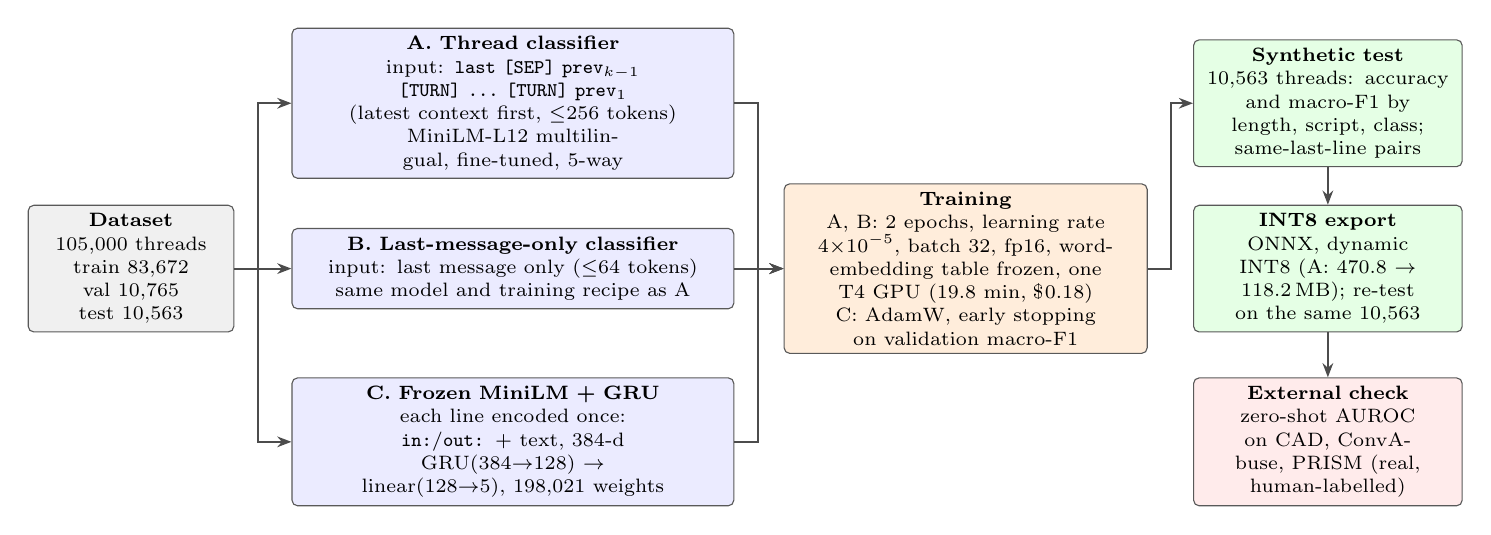
\begin{tikzpicture}
  \node[blk=gray!12, text width=2.4cm] (data) at (0.9,0) {\textbf{Dataset}\\105,000 threads\\train 83,672\\val 10,765\\test 10,563};
  \node[blk=blue!8, text width=5.4cm] (A) at (5.75,2.1) {\textbf{A. Thread classifier}\\input: \texttt{last [SEP] prev$_{k-1}$ [TURN] \dots\ [TURN] prev$_1$}\\(latest context first, $\le$256 tokens)\\MiniLM-L12 multilingual, fine-tuned, 5-way};
  \node[blk=blue!8, text width=5.4cm] (B) at (5.75,0) {\textbf{B. Last-message-only classifier}\\input: last message only ($\le$64 tokens)\\same model and training recipe as A};
  \node[blk=blue!8, text width=5.4cm] (C) at (5.75,-2.2) {\textbf{C. Frozen MiniLM + GRU}\\each line encoded once: \texttt{in:}/\texttt{out:} + text, 384-d\\GRU(384$\to$128) $\to$ linear(128$\to$5), 198,021 weights};
  \node[blk=orange!14, text width=4.4cm] (train) at (11.5,0) {\textbf{Training}\\A, B: 2 epochs, learning rate $4{\times}10^{-5}$, batch 32, fp16, word-embedding table frozen, one T4 GPU (19.8 min, \$0.18)\\C: AdamW, early stopping on validation macro-F1};
  \node[blk=green!10, text width=3.2cm] (test) at (16.1,2.1) {\textbf{Synthetic test}\\10,563 threads: accuracy and macro-F1 by length, script, class; same-last-line pairs};
  \node[blk=green!10, text width=3.2cm] (int8) at (16.1,0) {\textbf{INT8 export}\\ONNX, dynamic INT8 (A: 470.8 $\to$ 118.2\,MB); re-test on the same 10,563};
  \node[blk=red!8, text width=3.2cm] (ext) at (16.1,-2.2) {\textbf{External check}\\zero-shot AUROC on CAD, ConvAbuse, PRISM (real, human-labelled)};
  \draw[arr] (data.east) -- ++(3mm,0) |- (A.west);
  \draw[arr] (data.east) -- (B.west);
  \draw[arr] (data.east) -- ++(3mm,0) |- (C.west);
  \draw[arr] (A.east) -- ++(3mm,0) |- (train.west);
  \draw[arr] (B.east) -- (train.west);
  \draw[arr] (C.east) -- ++(3mm,0) |- (train.west);
  \draw[arr] (train.east) -- ++(3mm,0) |- (test.west);
  \draw[arr] (test.south) -- (int8.north);
  \draw[arr] (int8.south) -- (ext.north);
\end{tikzpicture}
}
  \caption{Models, training and evaluation. A and B are fine-tuned end to end; C keeps the encoder frozen and trains only a GRU \cite{cho2014gru} over per-line vectors.}
  \label{fig:training}
\end{figure*}

\par\textbf{Model A (thread).} The input is the last message followed by the earlier messages in reverse order, separated by \texttt{[TURN]}, truncated to 256 tokens (from the earlier messages if too long). \textbf{Model B (last message only)} sees only the last message (64 tokens). Both are fine-tuned for 2 epochs (learning rate $4\times10^{-5}$, batch 32, fp16) with the 250k-token word-embedding table frozen to save memory, on one NVIDIA T4 GPU (AWS g4dn.xlarge, 19.8 minutes, \$0.18). Validation used a random subset of 4{,}000 validation threads. \textbf{Model C} encodes each line once with the frozen encoder (prefix \texttt{in:} for the speaker of the last message, \texttt{out:} for the other; mean pooling, 384 numbers), runs a one-layer forward GRU (hidden size 128) over the vectors, and a linear layer gives 5 scores. It has 198{,}021 weights. As a control we also trained C on the last line's vector alone.

\par\textbf{INT8 export.} Models A and C's encoder were exported to ONNX and dynamically quantized to INT8 (Section~\ref{sec:binary}); both are 118\,MB. The INT8 files were re-tested on the same test set.

\par\textbf{Metrics.} \emph{Accuracy} is the share of correctly classified test threads. \emph{Macro-F1} is the mean of the five per-class F1 scores. We report both by length, by script and per class (recall), and \emph{pair accuracy} on the 2{,}337 same-last-line test threads. On external data we report \emph{AUROC} of the score $P(\text{hostile})+P(\text{harassment})$ against a binary abusive label (Section~\ref{sec:external}).

%==============================================================
\section{Results on the Synthetic Test Set}\label{sec:results}
Table~\ref{tab:main_results} gives the main numbers on the 10{,}563 held-out synthetic threads.

\begin{table*}[t]
\centering
\caption{Five-class results on the synthetic test set (10{,}563 threads). Acc.\ in \%; by-length columns are accuracy. Pairs: same-last-line threads (2{,}337).}
\label{tab:main_results}
\small
\begin{tabularx}{\textwidth}{@{}l r R R R R R R R R@{}}
\toprule
\textbf{Model} & \textbf{Size} & \textbf{Acc.} & \textbf{Macro-F1} & \textbf{Len 3} & \textbf{Len 5} & \textbf{Len 7} & \textbf{Len 10} & \textbf{Pairs} \\
\midrule
A. Thread, fine-tuned (FP32)           & 470.8\,MB & 97.96 & 0.980 & 96.9 & 98.4 & 98.2 & 98.4 & 97.4 \\
A. Thread, fine-tuned (INT8)           & 118.2\,MB & 97.88 & 0.979 & 96.9 & 98.3 & 98.1 & 98.3 & 97.5 \\
B. Last message only (FP32)            & $\approx$470.8\,MB & 83.18 & 0.828 & 85.1 & 84.1 & 82.7 & 80.8 & 51.3 \\
C. Frozen encoder + GRU (FP32)         & 470.2 + 0.8\,MB & 95.17 & 0.952 & 93.0 & 95.3 & 95.6 & 96.9 & 93.6 \\
C. Frozen INT8 encoder + GRU           & 118.1 + 0.8\,MB & 94.91 & 0.950 & 92.3 & 95.1 & 95.7 & 96.7 & 93.1 \\
C-control. Last-line vector only + GRU & 470.2 + 0.8\,MB & 78.13 & 0.784 & 80.6 & 79.6 & 77.3 & 74.9 & 49.9 \\
\bottomrule
\end{tabularx}
\end{table*}

\par\textbf{Reading the table.} (i)~Context is the signal: removing the earlier messages costs 14.8 points (A vs.\ B), and the last-message-only models are at chance (about 50\%) on the pair threads, as the design implies. This tells us the benchmark requires context, not that the models understand it beyond this synthetic distribution. (ii)~Accuracy of B falls with length (85.1\% $\to$ 80.8\%) while A does not, because longer threads dilute a single-message cue. (iii)~INT8 quantization costs 0.08 points for A and 0.26 points for C. (iv)~The frozen encoder with a GRU trails fine-tuning by 2.8 points, and its GRU part is tiny (4\,MB as JSON), but the multilingual word-embedding table makes the INT8 encoder about 118\,MB either way.

\par\textbf{By script and class (A, INT8).} Accuracy is 99.3\% in English, 97.5\% in Hindi and 96.9\% in Hinglish. Per-class recall is 97.4\% (benign), 96.3\% (friendly\_sarcasm), 98.1\% (hostile\_abuse), 98.1\% (sexual\_harassment) and 99.8\% (predatory\_grooming). The most common errors are friendly\_sarcasm and hostile\_abuse confused with each other (59 and 32 test threads) and benign vs.\ sexual\_harassment (36 and 21).

\par\textbf{Latency of A (INT8).} With native ONNX Runtime (1 thread, batch 1, 256-token cap, 300 five-message Hinglish threads) the median is 28.3\,ms and the 95th percentile 37.0\,ms, including tokenization; this is again not an in-browser measurement.

%==============================================================
\section{External Validation on Real Data: a Negative Result}\label{sec:external}
To test whether the synthetic training transfers, we scored three real, human-labelled datasets \emph{without fine-tuning}, using the FP32 models A and B (Table~\ref{tab:external}). Real data lack our five classes, so we mapped them to \emph{abusive} (score $=P(\text{hostile})+P(\text{harassment})$) vs.\ not. AUROC is 0.5 for chance and 1.0 for perfect.

\begin{table}[t]
\centering
\caption{Zero-shot AUROC of the synthetic-trained models on real data. ``Last'' scores only the last message (model B); ``Thread'' uses earlier messages too (model A). PRISM has no threads.}
\label{tab:external}
\footnotesize
\begin{tabular}{@{}l r r r@{}}
\toprule
\textbf{Dataset} & $n$ & \textbf{Last} & \textbf{Thread} \\
\midrule
CAD (EN threads) \cite{vidgen2021cad}          & 21,681 & 0.590 & 0.560 \\
\quad abuse only in earlier messages           & 18,984 & 0.581 & 0.536 \\
ConvAbuse (EN chatbot) \cite{curry2021convabuse} & 3,941 & 0.724 & 0.738 \\
\quad sexual-harassment flag (210 pos.)        & 3,941  & 0.566 & 0.541 \\
PRISM Hindi \cite{prism2025}                    & 9,767  & 0.469 & -- \\
PRISM Hinglish \cite{prism2025}                 & 4,781  & 0.515 & -- \\
PRISM English \cite{prism2025}                  & 14,996 & 0.669 & -- \\
\bottomrule
\end{tabular}
\end{table}

The models do not transfer: AUROC is between 0.47 and 0.74, and on CAD earlier messages did not help (0.560 with context vs.\ 0.590 without). We found one concrete failure: very short neutral replies such as ``yes'' or ``how old are you'' received a hostile score of about 0.999, because in our data hostile threads often end in a short insult, so the models partly learned ``short last line $\Rightarrow$ hostile''. A second cause is a definition mismatch: abuse in CAD is mostly identity- or affiliation-directed and often contains no profanity, while our hostile class is mainly personal fights. We could not evaluate on real Hinglish or Hindi \emph{threads}: HASOC ICHCL needs a key from the organisers (we did not have one), and we found no open threaded Hindi data. PRISM Hindi and Hinglish are single messages, and its labels come from several source datasets, whose guidelines we did not inspect. Model C and the INT8 files were not run on these datasets.

%==============================================================
\section{Limitations}
\begin{itemize}
    \item \textbf{Synthetic, unreviewed data.} Labels are the intended class of an LLM prompt, filtered by regular expressions; no human checked label quality, fluency (especially Hindi and Hinglish) or realism. Quality of Hindi and Hinglish text was not measured.
    \item \textbf{Same-generator test set.} The 95--98\% scores are on text from the same generator and templates as the training data; 22\% of the test threads end in one of only 36 shared lines per script. They are not evidence of real-world accuracy (Section~\ref{sec:external}).
    \item \textbf{Binary model.} The shipped Hinglish data are machine-converted and less code-mixed than human Hinglish; the cloud-LLM comparison uses 20--80 examples per slice.
    \item \textbf{Deployment.} Latency was measured natively, not in the browser; the five-class models are not in the extension; we did not measure memory use.
    \item \textbf{Ethics.} The dataset contains synthetic abusive, harassing and grooming text, but no real people. Grooming threads use only non-sexual cues (secrecy, isolation, gifts, age probing) and the prompts exclude sexual content and slurs about protected groups; the validators check sexual and profane words but not slurs. Such data should only be used for building protective classifiers.
\end{itemize}

%==============================================================
\section{Conclusion}
\textit{SurakshaNet} shows that a 118\,MB INT8 multilingual model can score WhatsApp Web messages locally, that a simple window gate helps with abuse split across messages on our Hinglish test set, and that a five-class thread benchmark can separate models that use context from those that do not. It does not yet show that these models work on real conversations: zero-shot AUROC on real data is 0.47--0.74. The next steps are to remove the short-last-line shortcut from the generator, add real threaded training data with held-out evaluation, obtain real Hinglish threads (HASOC ICHCL), and evaluate the INT8 models in the browser. Code, generation scripts and evaluation reports are in the project repository\footnote{\url{https://github.com/PrathamGarg1/temporart}}.

\bibliographystyle{ACM-Reference-Format}
\bibliography{references}

\end{document}
